
\textbf{\underline{Третья глава}} посвящена разработке и исследованию самодельного преобразователя силы на основе Velostat.

Для определения геометрических и физико-механических свойств поверхности было решено использовать датчик силы на ноге робота. Рассмотрев различные варианты, по причине дешевизны и легкости производства в лабораторных условиях, было решено использовать пьзорезистивный тип датчика, основанный на материале Velostat \pic{fig:velostat_sensor.jpg}. Он является промежуточным слоем \pic{fig:simplest_sensor.jpg}. Электрическая схема \pic{fig:el_scheme}. 


\begin{figure}[ht]
    \begin{subfigure}[t]{0.45\textwidth}
        \centering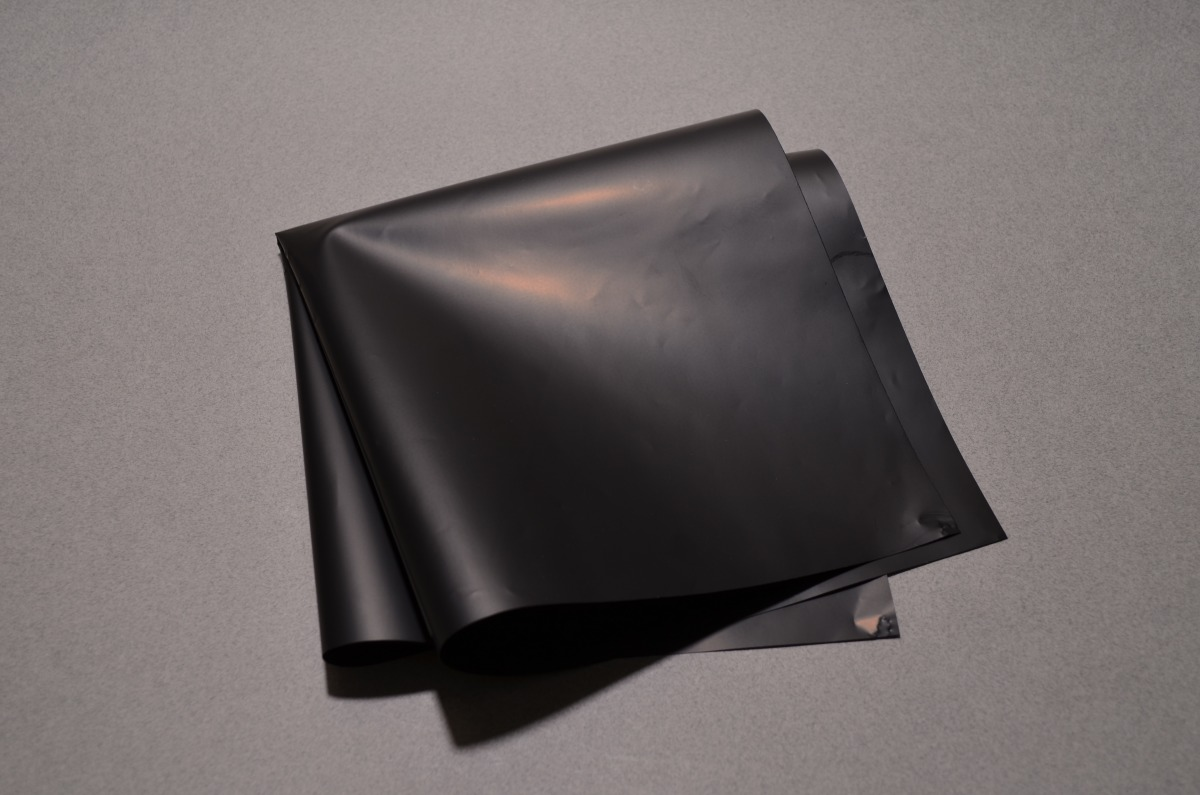
\includegraphics[height=2.5cm,width=1\textwidth,keepaspectratio]{velostat_sensor.jpg}
        \caption{Материал Velostat}
        \label{fig:velostat_sensor.jpg}
    \end{subfigure}
    \begin{subfigure}[t]{0.45\textwidth}
        \centering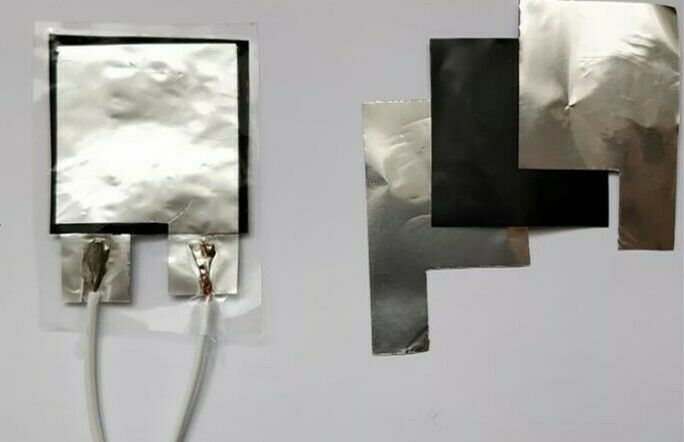
\includegraphics[height=2.5cm,width=1\textwidth,keepaspectratio]{simplest_sensor.jpg}
        \caption{Простейший преобразователь силы на основе Velostat}
        \label{fig:simplest_sensor.jpg}
    \end{subfigure}

    \begin{subfigure}[t]{0.9\textwidth}
        \centering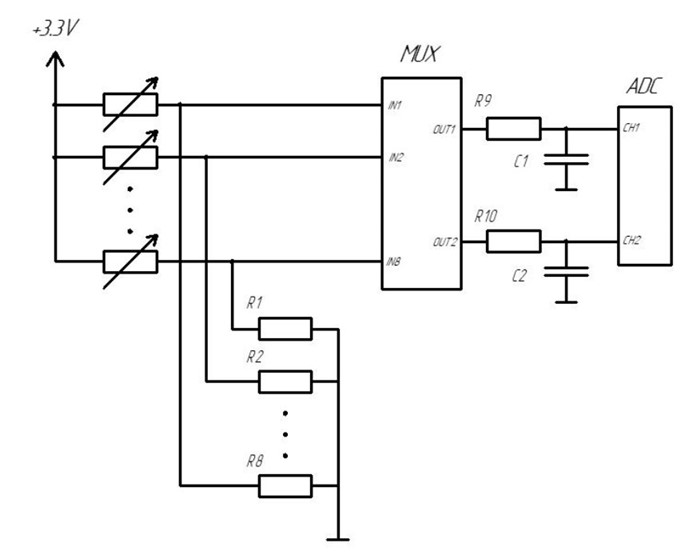
\includegraphics[height=4cm,width=1\textwidth,keepaspectratio]{electric_scheme.jpg}\\
        \caption{Электрическая схема преобразователя силы}
        \label{fig:el_scheme}
    \end{subfigure}
    \caption{Примеры использования Velostat}
\end{figure}

При исследовании преобразователя силы на основе Velostat, было замечено, что площадь нажатия влияет на показания преобразователя. 

Задача: охарактеризовать материал для случаев, когда нагрузка меньше, чем размер сенсора.

Давление на датчик приводит к изменению его сопротивления: чем выше давление, тем ниже сопротивление. На \pic{fig:velostat_pressure_resistance.jpg} показана рабочая область сенсора, основанная на весе, который может быть приложен на одну ногу робота.
\begin{figure}[h]
    \centering
    \begin{tikzpicture}
        % Include the image in a node
        \node [above right, inner sep=0] (image) at (0,0)
        {\centering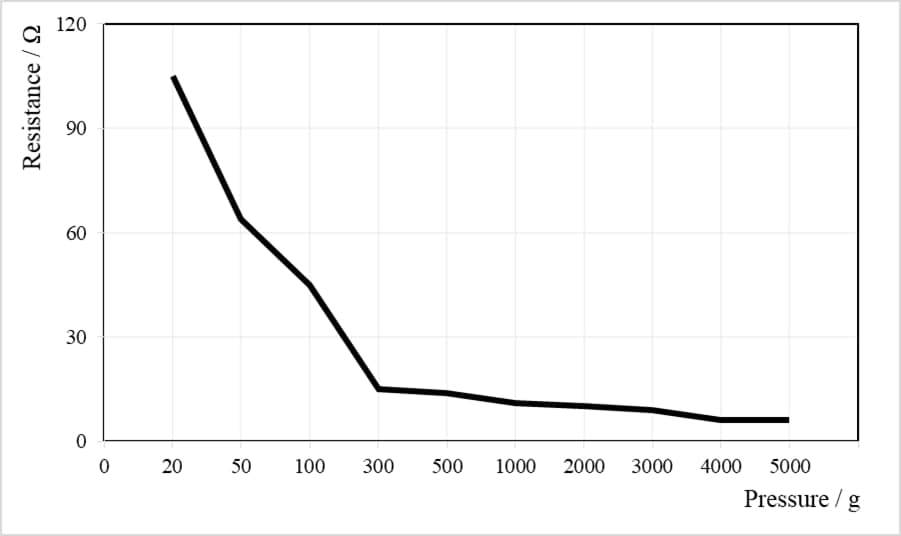
\includegraphics[height=3.5cm,width=1\textwidth,keepaspectratio]{velostat_pressure_resistance.jpg}};
        % Create scope with normalized axes
        \begin{scope}[
                x={($ 0.1*(image.south east)$)},
                y={($ 0.1*(image.north west)$)}]
            \draw[stealth-, very thick,green] (4.21,2.75) -- (6.5,5);
            \draw[stealth-, very thick,green] (8.75,2.15) -- (6.5,5)
            node[rounded corners=3pt,above,black,fill=white]{\small Рабочая область};
        \end{scope}
    \end{tikzpicture}
    \caption{График зависимости прикладываемого веса от сопротивления}
    \label{fig:velostat_pressure_resistance.jpg}
\end{figure}

Для исследования сенсора был сделан стенд. Требования: необходимость контролировать силу нажатия и обеспечить повторяемость эксперимента как по величине, так и по расположению площадки контакта инструмента и исследуемого преобразователя силы. 

Разработанный стенд, представлен на рисунке \ref{fig:exp_standd}.

\begin{figure}[ht]
    \begin{center}
            \begin{tikzpicture}
                % Include the image in a node
                \node [
                    above right,
                    inner sep=0] (image) at (0,0) {\centering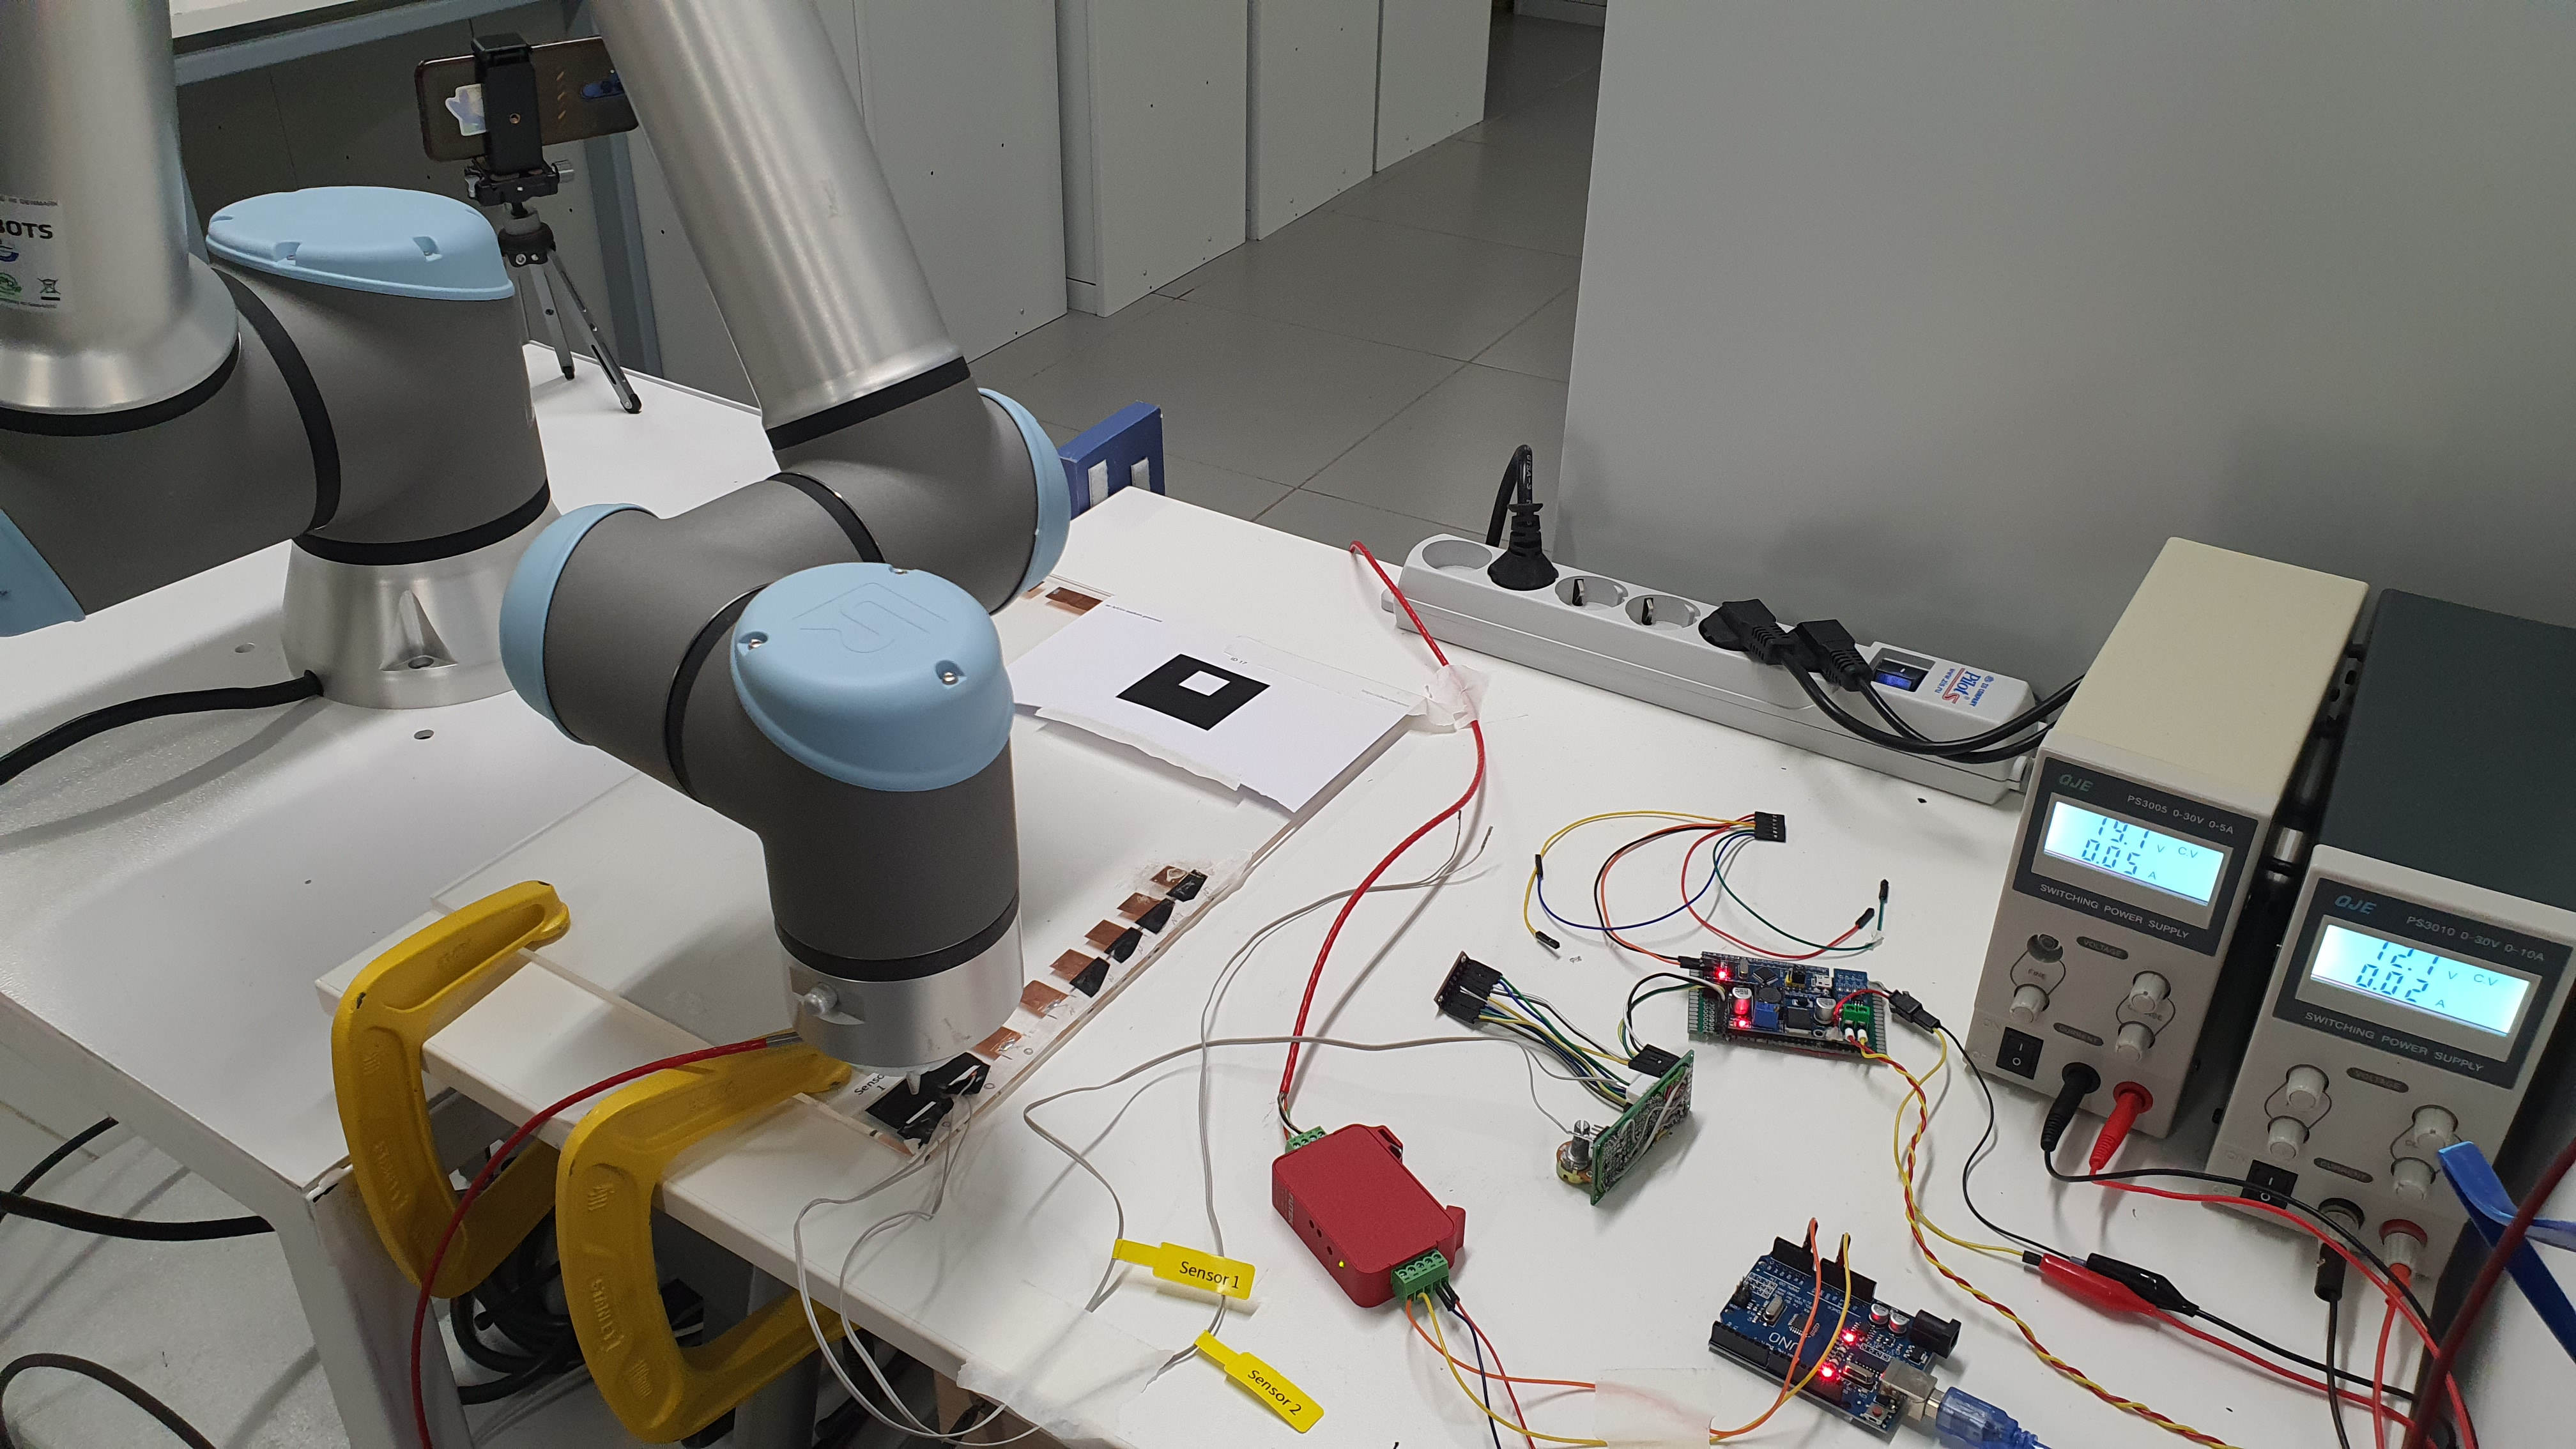
\includegraphics[height=5cm,width=1\textwidth,keepaspectratio]{exp_stand1}};

                % Create scope with normalized axes
                \begin{scope}[
                        x={($0.1*(image.south east)$)},
                        y={($0.1*(image.north west)$)}]
                    \draw[latex-, very thick,green] (3.5,2.2) -- (2.5,1)
                    node[rounded corners=3pt,below left,black,fill=white]{\small Velostat сенсор};

                    \draw[stealth-, very thick,green] (3.5,2.6) -- ++(-0.7,+0.5)
                    node[rounded corners=3pt,left,black,fill=white]{\small Датчик силы};

                    \draw[stealth-, very thick,green] (6.5,3) -- (7,6)
                    node[rounded corners=3pt,above right,black,fill=white]{\small Self-made PCB};

                    \draw[stealth-, very thick,green] (7.2,1.5) -- (8,5)
                    node[rounded corners=3pt,above right,black,fill=white]{\small Ардуино};

                    \draw[stealth-, very thick,green] (2.5,9.5) -- (4,9.5)
                    node[rounded corners=3pt,right,black,fill=white]{\small Камера};

                    \draw[very thick,green] (0.5,2.5) rectangle (4.2,9)
                    node[below left,black,fill=green]{\small UR10e};

                    \draw[latex-, very thick,green] (4.5,7.2) edge (5.5,7.5)
                    (4.8,5.3) -- (5.5,7.5)
                    node[rounded corners=3pt,above,black,fill=white]{\small Aruco маркеры};
                \end{scope}
            \end{tikzpicture}
        
        \caption{Разработанный экспериментальный стенд}
        \label{fig:exp_standd}
    \end{center}
\end{figure}

Для касания только части объекта исследования были разработаны различные насадки. Минимальный размер препятствия, который может коснуться робот было взято за 2 мм. Длина ребра датчика -- 15 мм \pic{fig:all_end_effectors.png}.

\begin{figure}[ht]
    \begin{subfigure}{0.6\textwidth}
        \centering
        \begin{tikzpicture}
            % Include the image in a node
            \node [above right, inner sep=0] (image) at (0,0)
            {\centering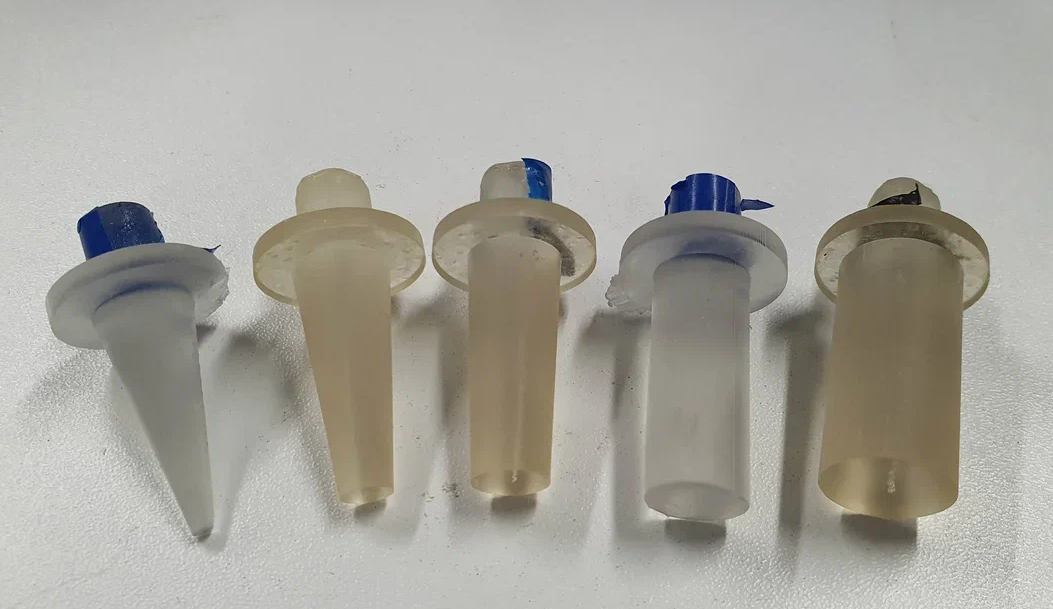
\includegraphics[height=3.5cm,width=1\textwidth,keepaspectratio]{all_end_effectors.png}};
            % Create scope with normalized axes
            \begin{scope}[
                    x={($ 0.1*(image.south east)$)},
                    y={($ 0.1*(image.north west)$)}]
                \node[rounded corners=3pt,black,fill=white] at (1.1,7.4){\tiny 2 мм };
                \node[rounded corners=3pt,black,fill=white] at (3.1,7.9){\tiny 6 мм };
                \node[rounded corners=3pt,black,fill=white] at (4.9,8.1){\tiny 8 мм };
                \node[rounded corners=3pt,black,fill=white] at (6.7,7.9){\tiny 12 мм };
                \node[rounded corners=3pt,black,fill=white] at (8.6,7.9){\tiny 15 мм };
            \end{scope}
        \end{tikzpicture}
        \caption{Насадки для нажатия на сенсор}
        \label{fig:all_end_effectors.png}
    \end{subfigure}
    \begin{subfigure}{0.38\textwidth}
        \centering
        \begin{tikzpicture}

            % Include the image in a node
            \node [
                above right,
                inner sep=0] (image) at (0,0) {\centering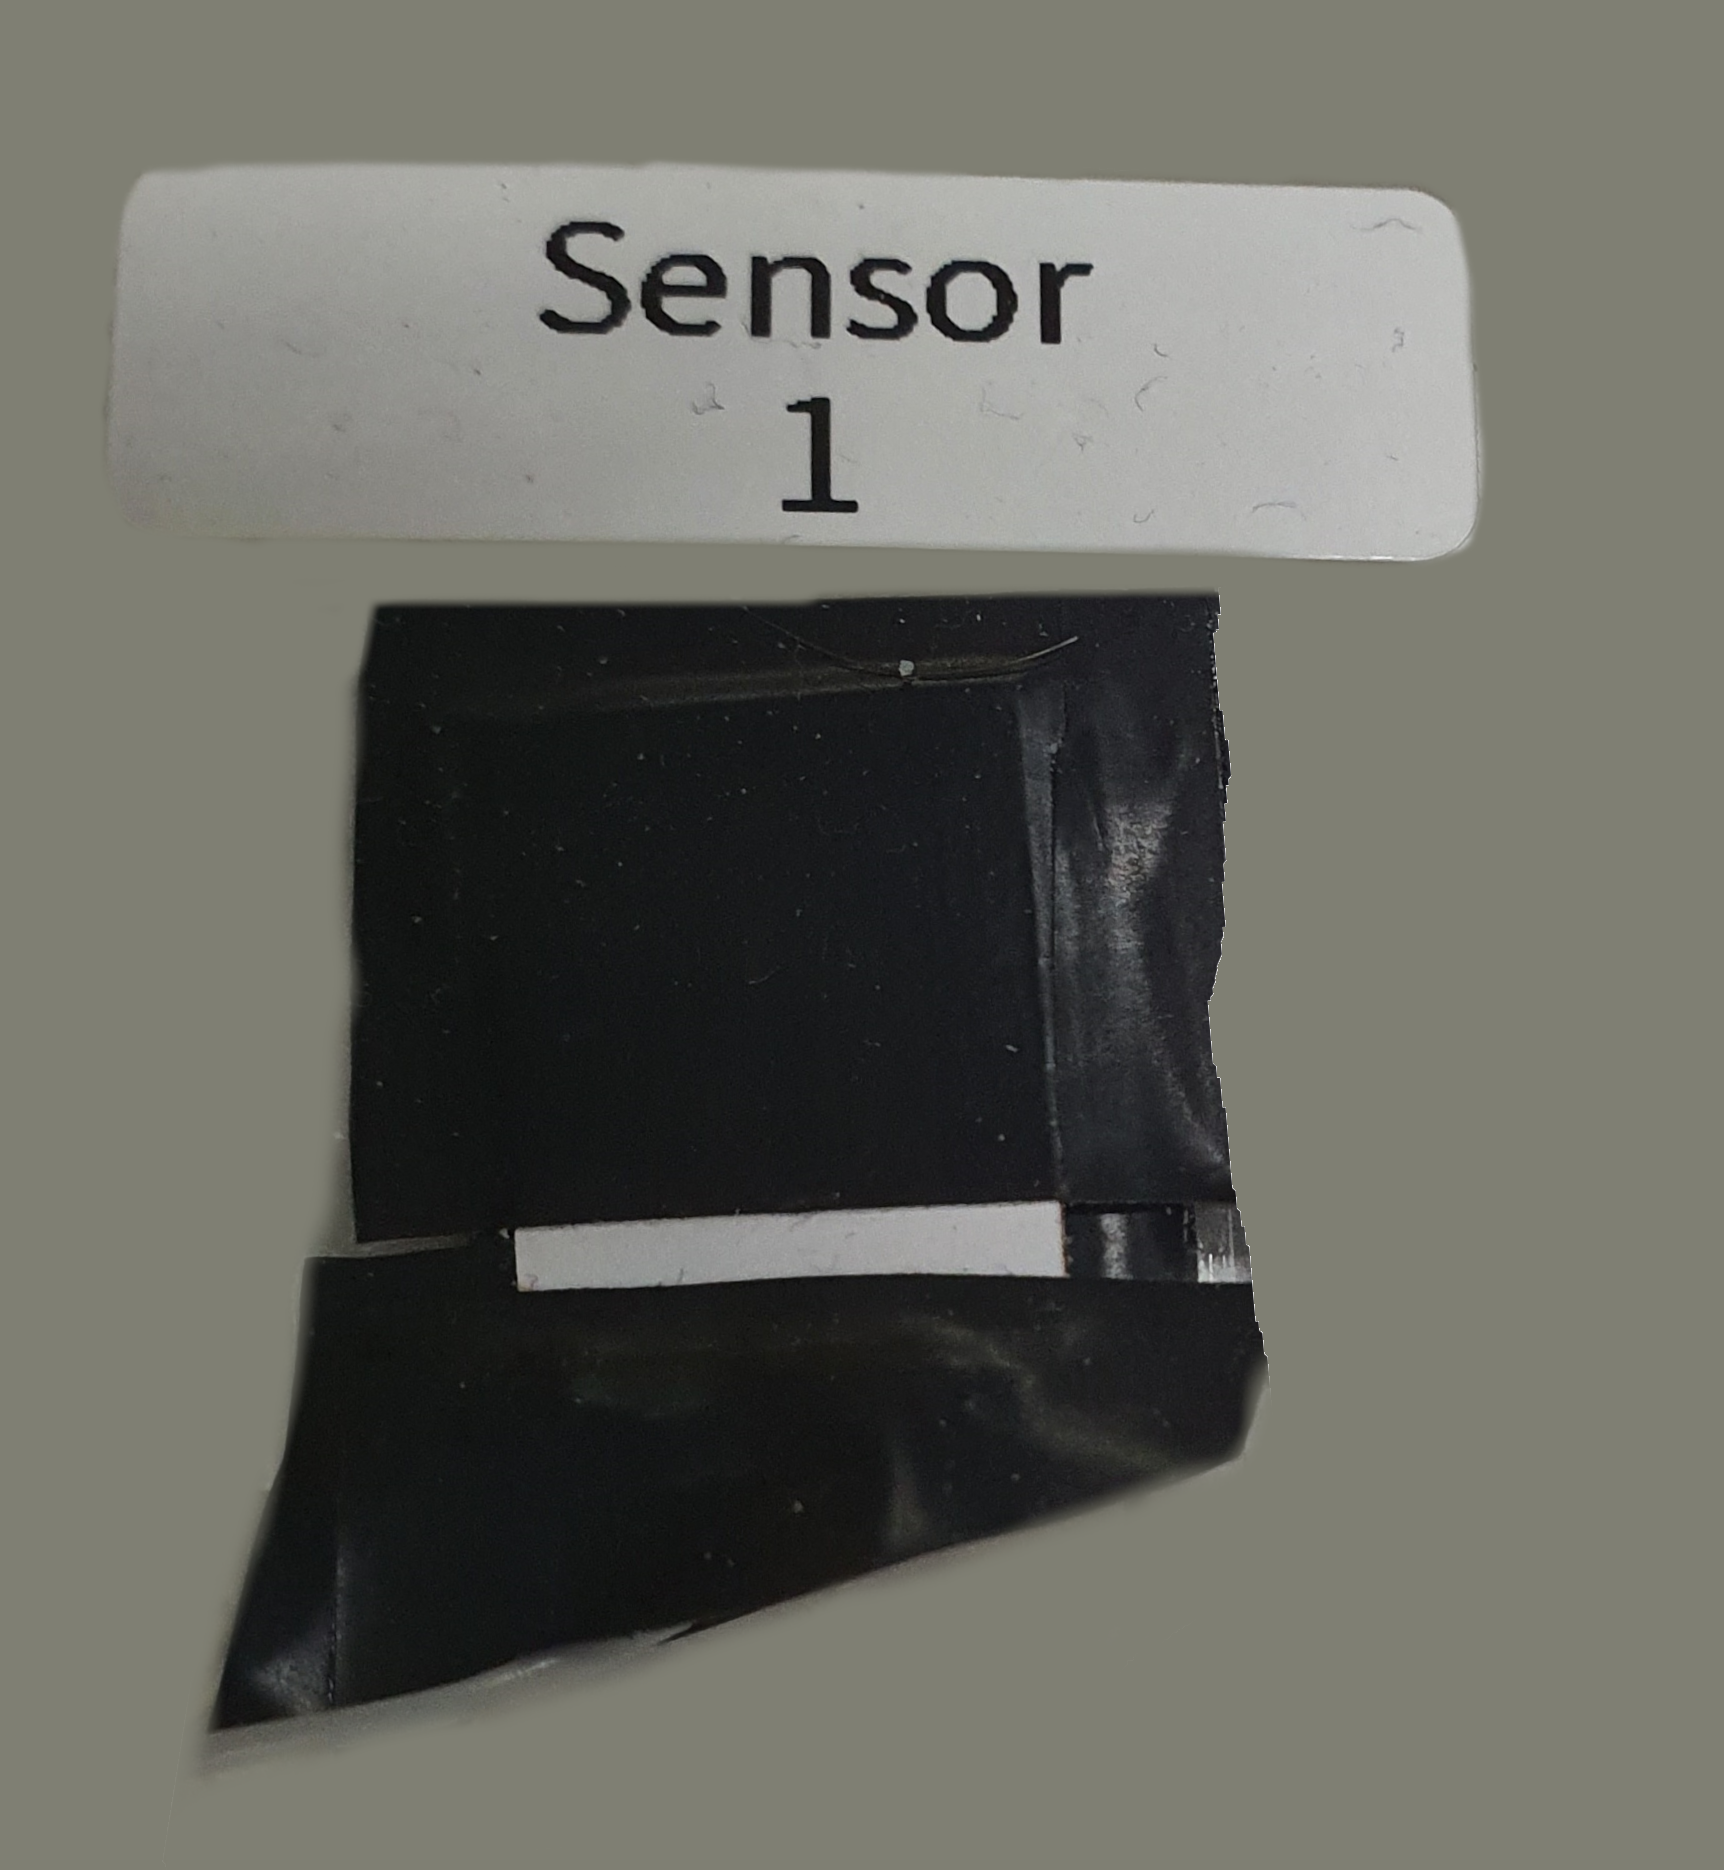
\includegraphics[height=3.5cm,width=1\textwidth,keepaspectratio]{sensors_grid.png}};

            % Create scope with normalized axes
            \begin{scope}[
                    x={($0.1*(image.south east)$)},
                    y={($0.1*(image.north west)$)}]
                \draw [green, very thick,
                    decorate,
                    decoration = {brace,
                            raise=5pt,
                            amplitude=5pt,
                            aspect=0.5}] (6,3.7) --  (3,3.7)
                node[pos=0.5,below=10pt,green]{$15$ мм};

                \draw [green, very thick,
                    decorate,
                    decoration = {brace, mirror,
                            raise=5pt,
                            amplitude=5pt,
                            aspect=0.5}] (6,3.6) --  (6,6.4)
                node[pos=0.5,right=10pt,green]{$15\ $ мм};

                \draw[green,step=1,xshift=22, yshift=30]  (0.5,0.5) grid +(3,3);

                \node[circle,fill=green,scale=0.4] at (3.3,6.27){\small 1};
                \node[circle,fill=green,scale=0.4] at (5.92,3.7){\small 16};
            \end{scope}

        \end{tikzpicture}
        \caption{Сенсор представлен \\ как $4\times4$ сетка}
        \label{fig:sensor_grid}
    \end{subfigure}
    \caption{Представление места нажатия инструментом сенсора и сам инструмент}
\end{figure}

Для контролирования силы нажатия манипулятором сенсора, было реализовано импедансное управление \pic{fig:force_data_pos.png}. Результат работы на частоте 450 $Hz$, необходимая сила нажатия --- $17\ H$.
\begin{figure}[h]
        \centering
         \begin{tikzpicture}
            % Include the image in a node
            \node [above right, inner sep=0] (image) at (0,0) 
            {\centering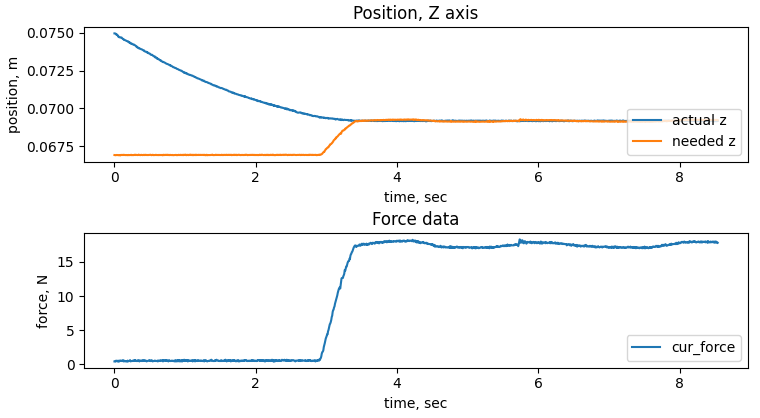
\includegraphics[height=5cm,width=1\textwidth,keepaspectratio]{force_data_pos.png}};          
            % Create scope with normalized axes
            \begin{scope}[
                x={($ 0.1*(image.south east)$)},
                y={($ 0.1*(image.north west)$)}]
                \draw[thick,green, dashed] (4.2,1) -- (4.2,8)
                node[above right,black,fill=white]{\tiny Касание с поверхностью};
            \end{scope}
        \end{tikzpicture}
        \caption{Графики зависимости силы и позиции по $z$ от времени во время эксперимента по исследованию Velostat}
        \label{fig:force_data_pos.png}
    \end{figure}

Было проведено 2 эксперимента. В \textbf{статическом} --- задача определить коэффициенты для математической модели преобразователя (калибровка датчика). На сенсор прикладывается известная нагрузка на 60 секунд (за это время можно явно наблюдать гистерезис) и собираются данные с преобразователя.

Для калибровки использовалась формула \eqref{eq:velostat_eqn}. Из-за гистерезиса необходимо учитывать время нажатия на объект, так как показания сенсора меняются со временем.
\begin{align}
    \label{eq:velostat_eqn}
    V_{out} = V_0 + p[k_p + k_e(1-e^\frac{-(t-t_0)}{\tau_{res}})](1-e^{-\frac{A}{p}}) \\
    k_p = A_1e^{-A_2p}; \tau_{res} = B_0 + B_1e^{-\frac{p}{B_2}}
\end{align}
где,  $V_0$- начальное напряжение,$p,\ A_i,\ B_i,\ \tau_{res},\ k_i$  - настраиваемые константы, $t$ - текущее время, $t_0$ - время начала нажатия.
Для решения задачи регрессии использовался робастный нелинейный алгоритм наименьших квадратов. Результат представлен ниже \pic{fig:least_square_model.png}.

\begin{figure}[H]
    \centering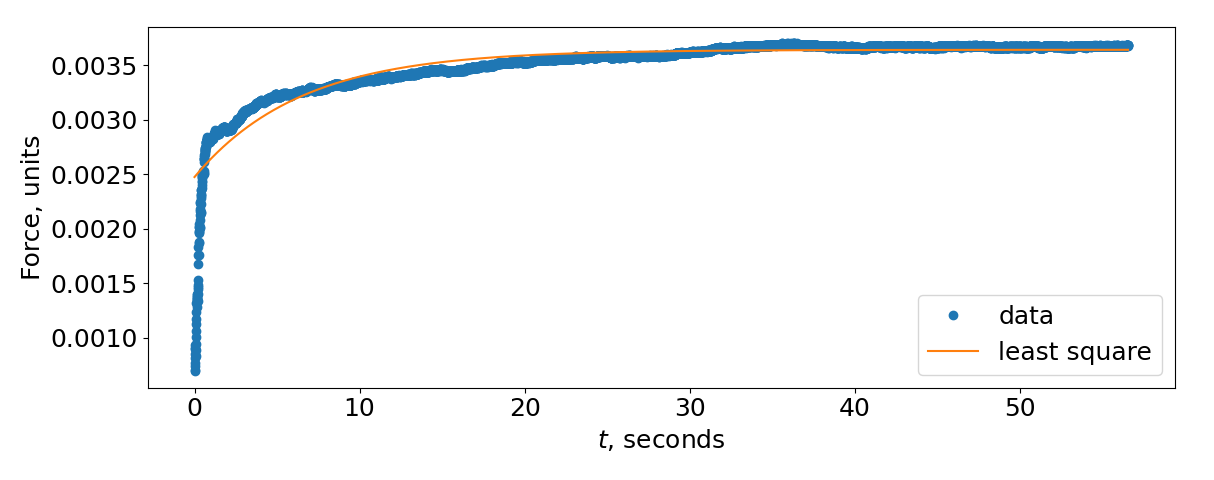
\includegraphics[height=2.8cm,width=1\textwidth,keepaspectratio]{least_square_model.png}
    \caption{Результаты статического эксперимента}
    \label{fig:least_square_model.png}
\end{figure}

\textbf{Динамический эксперимент}. Цель --- определить влияние показаний сенсора в зависимости от положения площадки контакта. Для этого преобразователь представлен в виде матрицы $4 \times 4$. Размер преобразователя в эксперименте 15 на 15 мм. Манипулятор нажимает на преобразователь с одинаковым давлением на протяжении всех экспериментов в различные позиции на преобразователе, используя пять различных концевых эффекторов (диаметр окружности от 2 мм до 15 мм) \pic{fig:sensor_grid}.



Ниже \pic{fig:dynamics_exp} представлены результаты распределения ошибок по площади сенсора при взаимодействии с насадками разных размеров. Ошибки определялись как разница между показаниями калиброванного сенсора силы Futek и исследуемого преобразователя на базе Velostat. На рисунке \ref{fig:sens1_pike1} показаны ошибки для насадки диаметром 2 мм, а на рисунке \ref{fig:sens1_pike3} --- диаметром 8 мм.

Можно заметить, что в \ref{fig:sens1_pike3} максимальная разница между Futek и Velostat не более 0.2 единиц в одном месте. Остальные элементы сетки не превышают 10\%. Такая же тенденция продолжается как и при увеличении размера насадки.

\begin{figure}[H]
    \begin{subfigure}{0.49\textwidth}
        \centering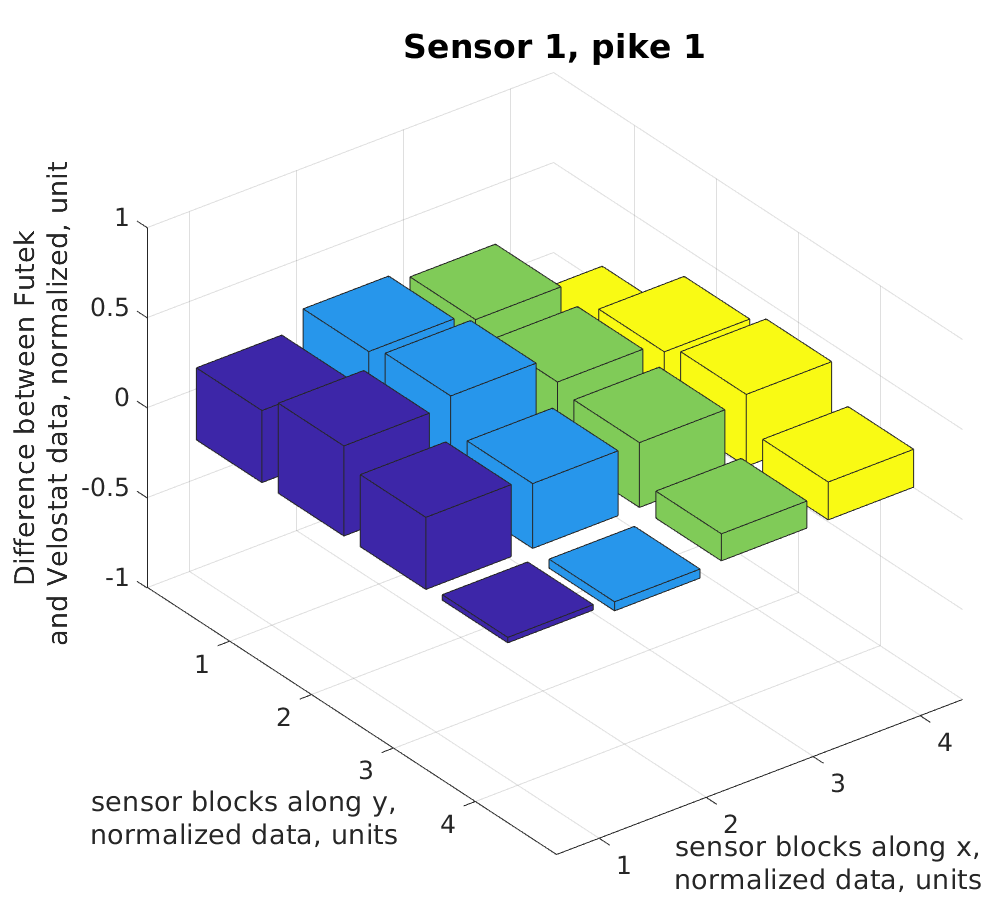
\includegraphics[height=4cm,width=1\textwidth,keepaspectratio]{sens1_pike1.png}
        \caption{Диаметр насадки равный 2 мм }
        \label{fig:sens1_pike1}
    \end{subfigure}
    \begin{subfigure}{0.49\textwidth}
        \centering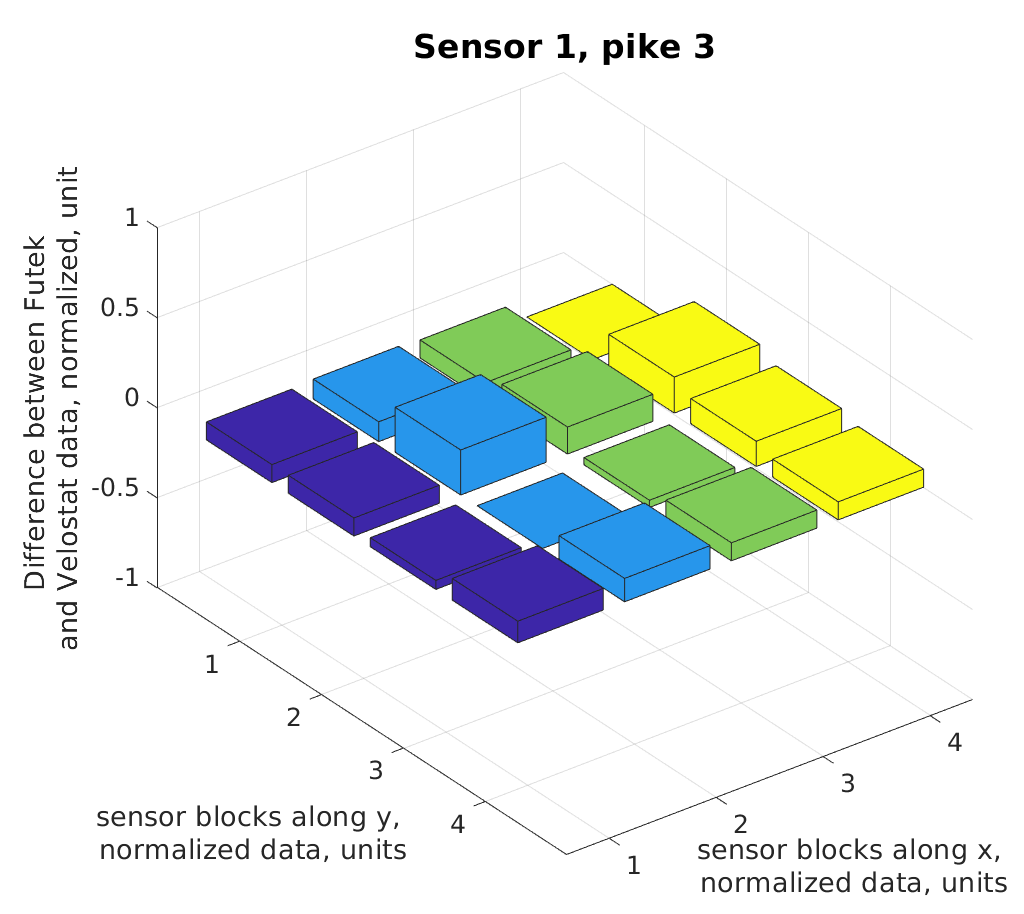
\includegraphics[height=4cm,width=1\textwidth,keepaspectratio]{sens1_pike3.png}
        \caption{Диаметр насадки равный 8 мм }
        \label{fig:sens1_pike3}
    \end{subfigure}
    \caption{Динамический эксперимент}
    \label{fig:dynamics_exp}
\end{figure}

По результатам исследований показано, что характеристики преобразователя удовлетворяют требованиям к системе тактильного восприятия шагающего робота, когда ожидаемый размер площади контакта превышает 25 процентов площади преобразователя.